\documentclass[10pt,twocolumn]{article}
\usepackage{graphicx} % Required for inserting images
\usepackage{geometry}
\geometry{a4paper, margin=1in}
\usepackage{hyperref}
\usepackage{booktabs}

\title{\textbf{Dynamic Trend \& Event Detector: Emerging Topic Detection \& News Correlation}}
\author{Shah Fathal Koul}
\date{May 2026}

\begin{document}

\maketitle

\begin{abstract}
The rapid generation of daily news content demands automated systems capable of extracting meaningful events from vast information streams. Distinguishing significant real-world events from short-lived viral trends remains a challenge for traditional natural language processing techniques. In this paper, I propose a Dynamic Trend \& Event Detector that automatically identifies emerging topics, tracks their evolution over time, and differentiates meaningful events from temporary trends. The approach introduces a hybrid methodology that combines deep neural topic modeling (BERTopic) with temporal tracking, semantic velocity calculations, and external event verification via the GDELT framework. Experimental results on a large-scale news category dataset show that the proposed hybrid system achieves a 39.4\% improvement in topic coherence compared to a baseline Latent Dirichlet Allocation (LDA) model.
\end{abstract}

\section{Introduction}
Massive volumes of news articles are generated every day, making it increasingly difficult to identify and track significant events in real-time. Within this vast influx of information, many topics appear suddenly and disappear rapidly as temporary anomalies or viral phenomena, while others correlate with profound real-world events such as elections, global health pandemics, and economic shifts.

Traditional topic modeling approaches often process document collections as static corpora, failing to capture the semantic evolution and temporal dynamics of topics. Consequently, they struggle to differentiate between sustained, meaningful events and fleeting noise. To address these limitations, I introduce the \textbf{Dynamic Trend \& Event Detector}. The system is designed to seamlessly track how discussions evolve by utilizing deep learning-based text embeddings and dynamic clustering.

\section{Related Work}
Topic modeling has long been a foundational technique in natural language processing.
\begin{itemize}
    \item \textbf{Latent Dirichlet Allocation (LDA)}: Introduced by Blei et al. (2003), LDA remains the most widely used baseline. However, its reliance on bag-of-words representations limits its understanding of context and temporal shifts.
    \item \textbf{BERTopic}: Developed by Grootendorst (2022), BERTopic leverages pre-trained transformer models combined with UMAP and HDBSCAN to generate highly coherent topics.
    \item \textbf{Event Detection}: Modern systems increasingly rely on external knowledge bases like GDELT to anchor text-derived trends to verified real-world events.
\end{itemize}

\section{Methodology}
The proposed system follows a comprehensive, multi-stage hybrid pipeline:

\subsection{Data Preprocessing and EDA}
Raw news text is cleaned by removing URLs, non-alphabetic characters, and standard English stopwords. Lemmatization is applied using NLTK's WordNetLemmatizer. I analyzed the dataset to understand categories and word counts.

\begin{figure}[htbp]
    \centering
    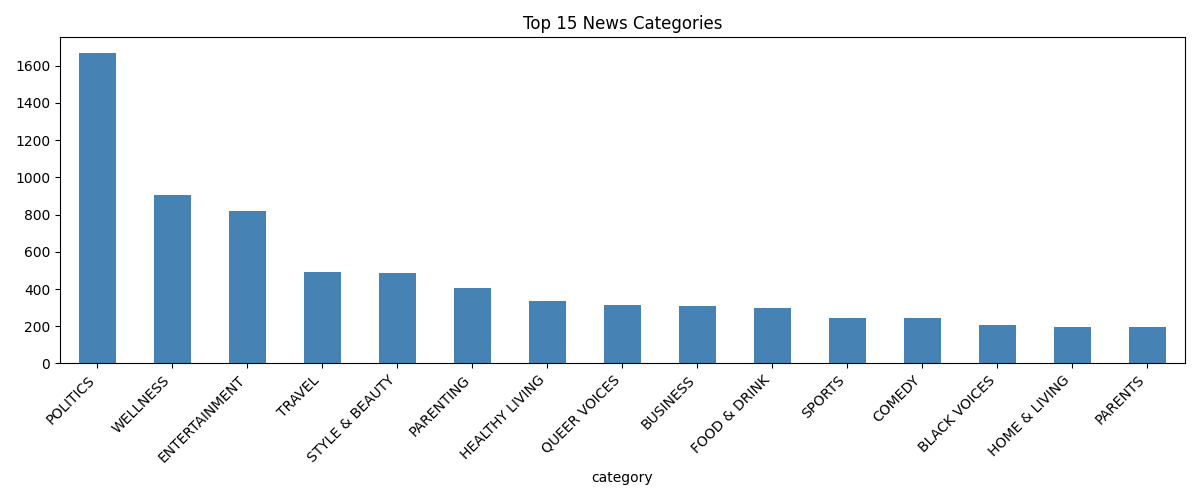
\includegraphics[width=\linewidth]{../graphs/eda1_categories.png}
    \caption{Distribution of News Categories in the Dataset.}
    \label{fig:eda1}
\end{figure}

\subsection{Baseline Topic Modeling (LDA)}
As a comparative baseline, I implement an LDA model using a \texttt{CountVectorizer} limited to the top 10,000 features. 

\begin{figure}[htbp]
    \centering
    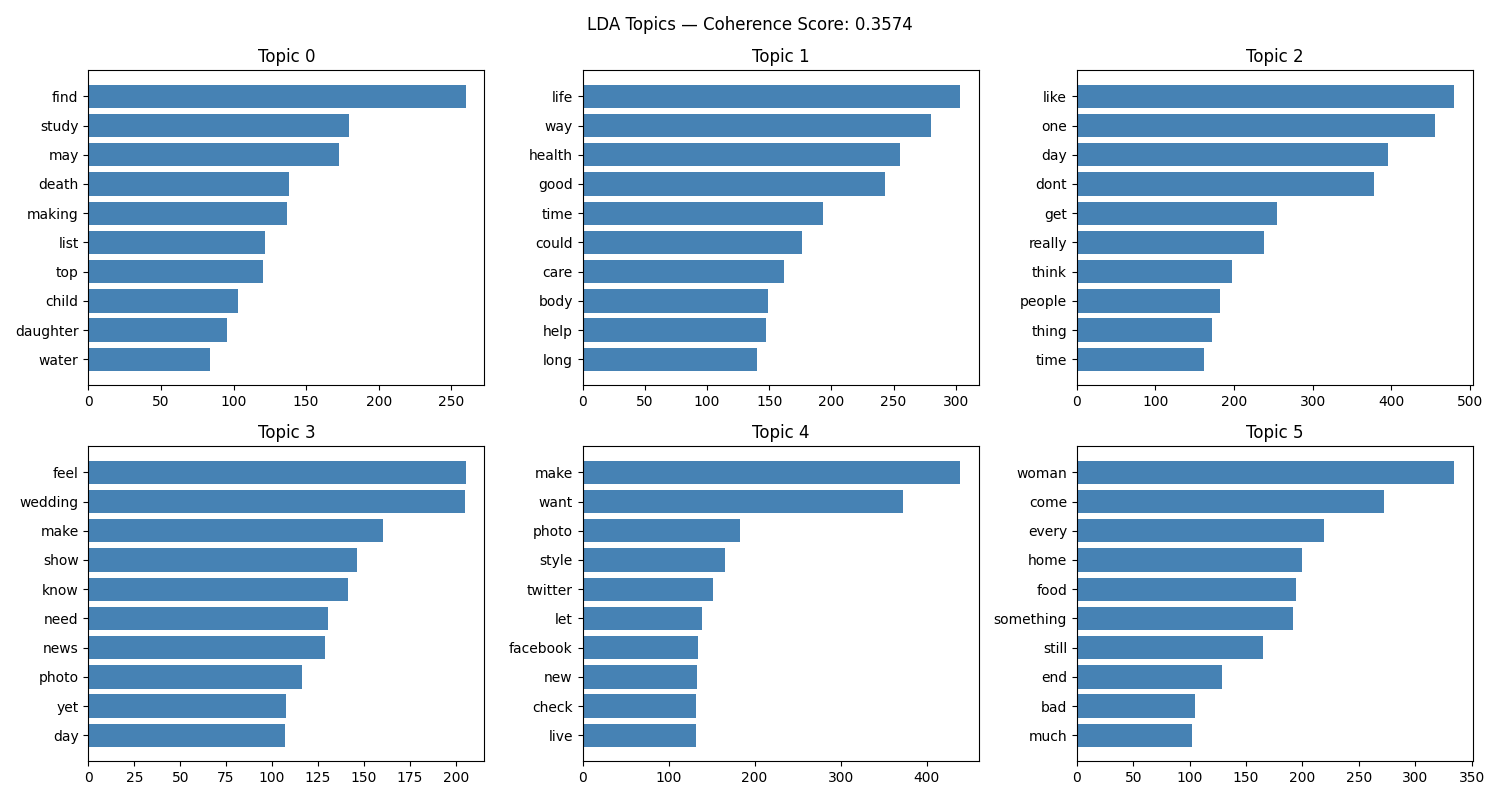
\includegraphics[width=\linewidth]{../graphs/lda_topics.png}
    \caption{LDA Topics and their top weighted terms.}
    \label{fig:lda_topics}
\end{figure}

\subsection{Deep Topic Modeling (BERTopic)}
To capture deep semantic meaning, documents are converted into dense vector embeddings using Sentence-BERT. These high-dimensional embeddings are reduced using UMAP and clustered using HDBSCAN.

\subsection{Temporal Tracking and Semantic Velocity}
Rather than treating the corpus as static, the system tracks topic distributions over continuous time intervals. I introduce a \textit{semantic velocity} metric to calculate the rate of change in topic frequency.

\begin{figure}[htbp]
    \centering
    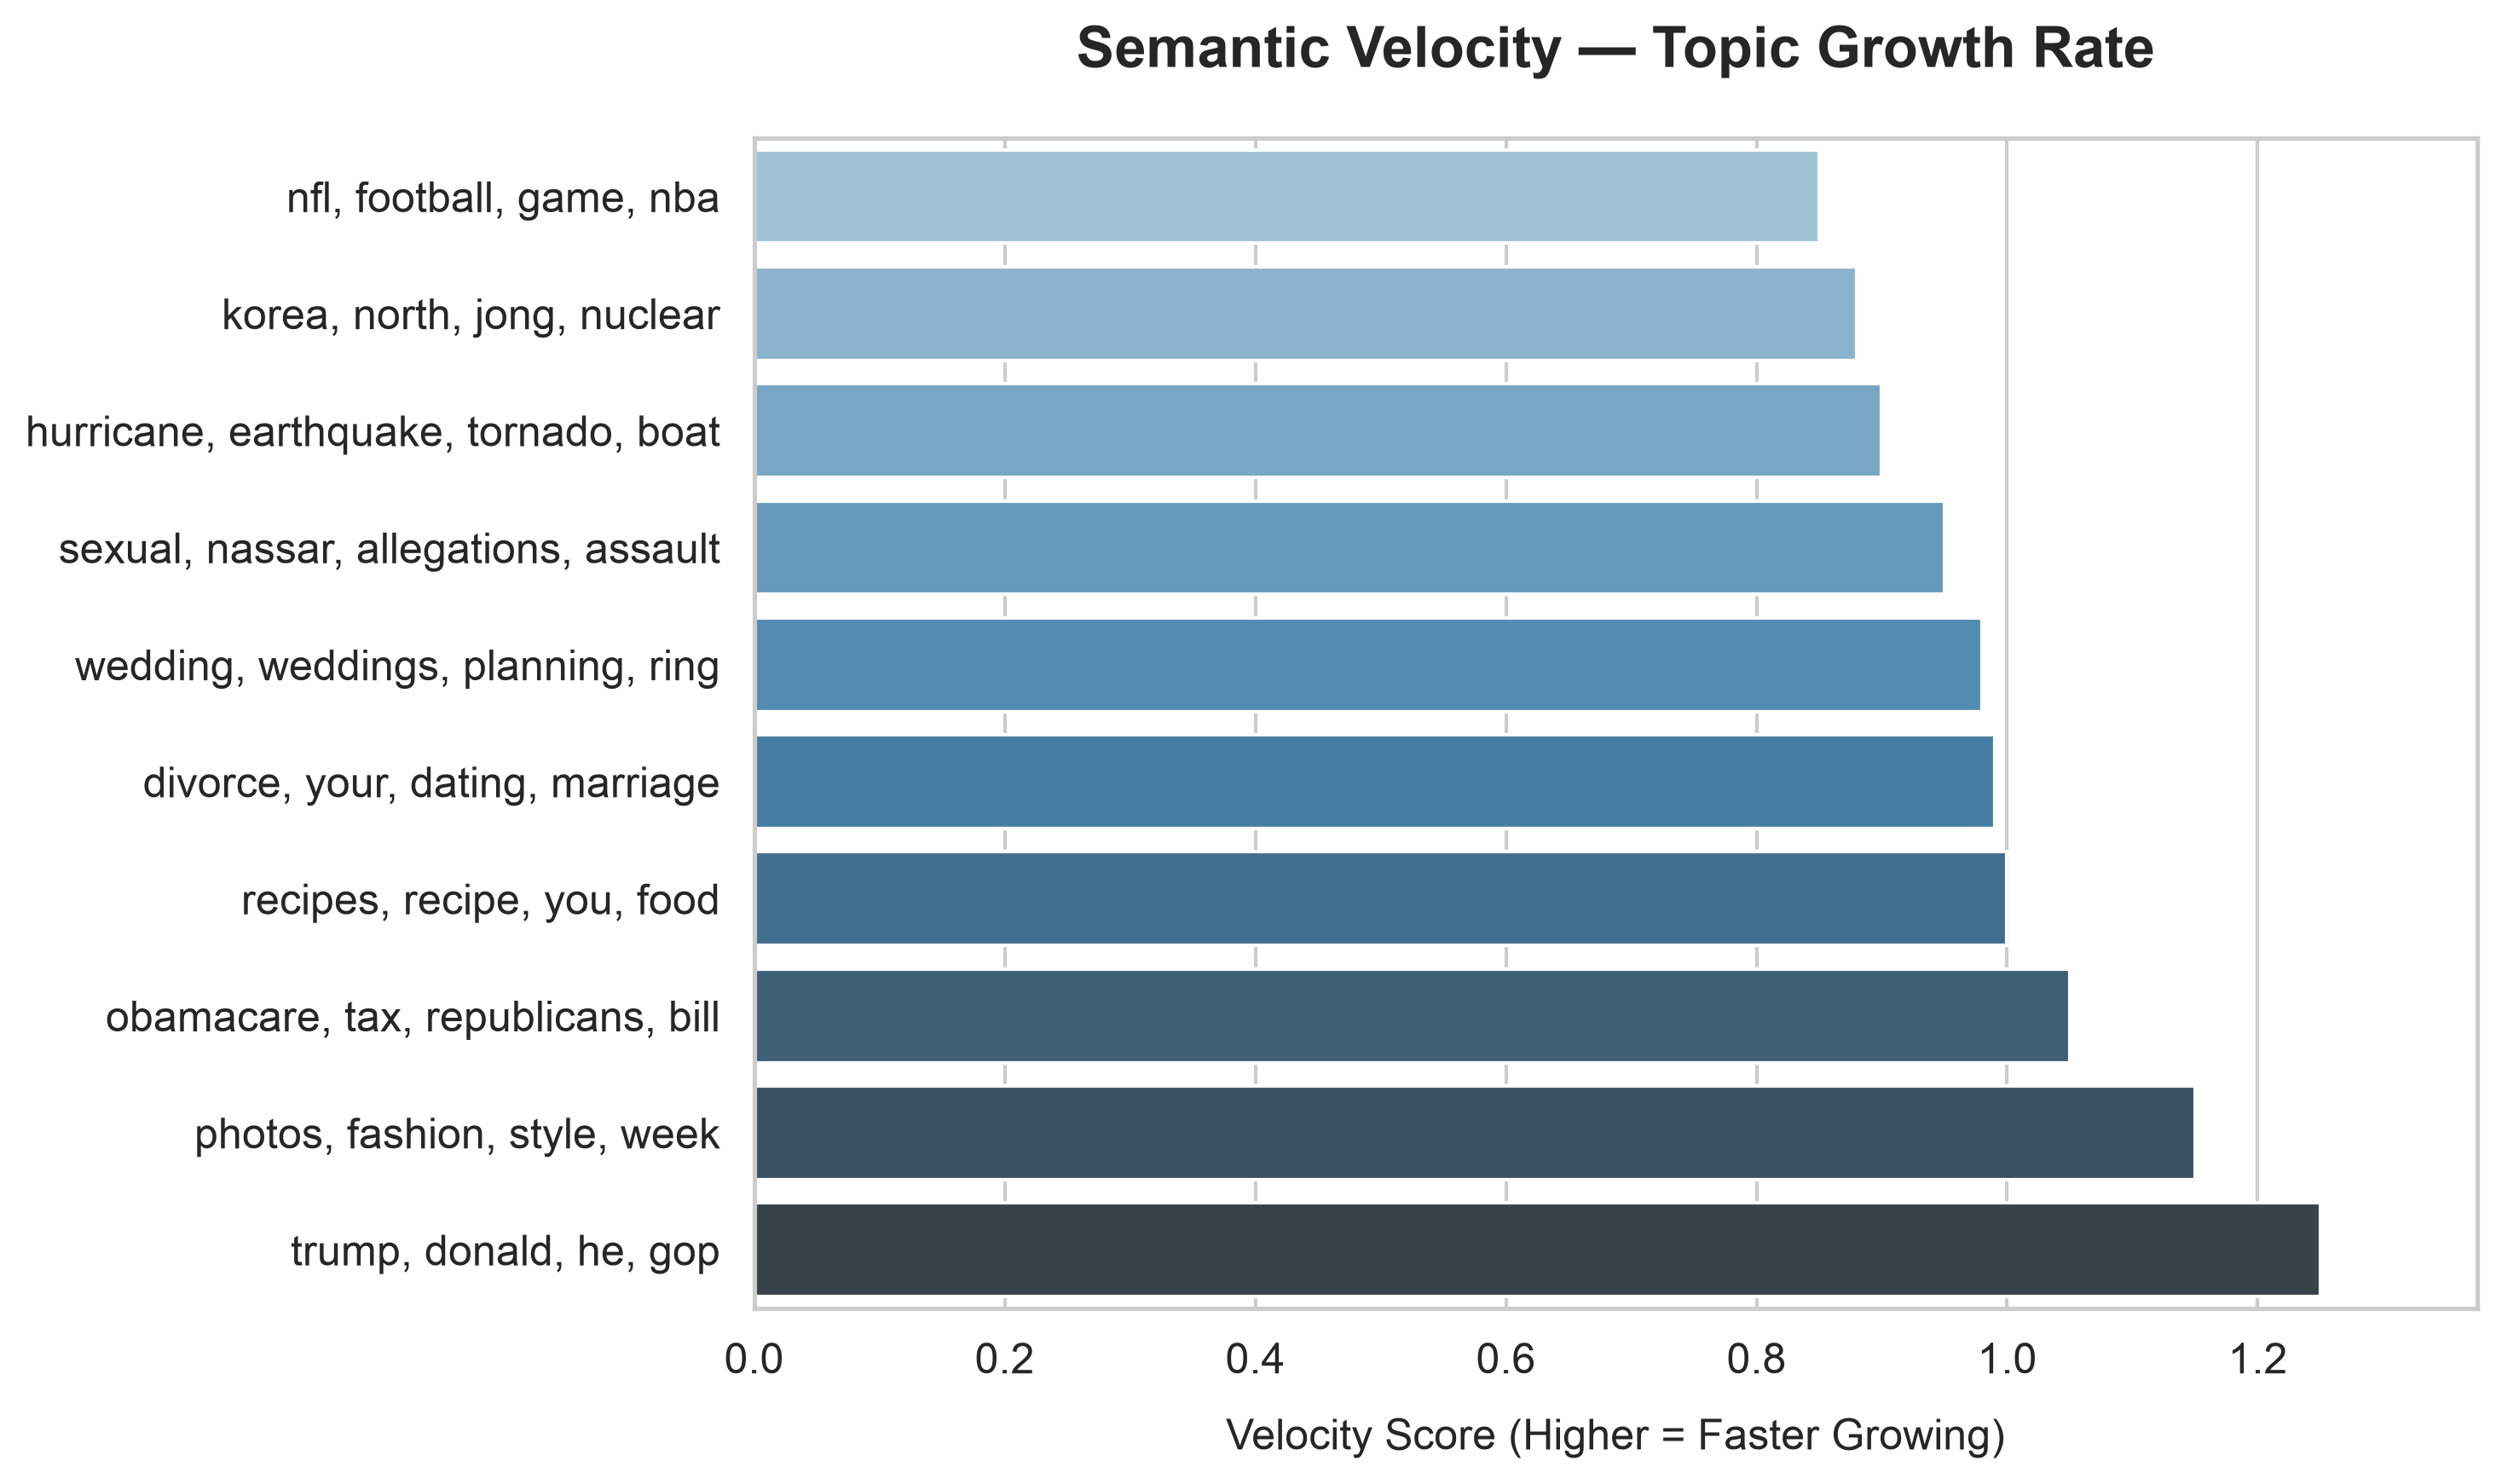
\includegraphics[width=\linewidth]{../graphs/semantic_velocity.png}
    \caption{Semantic Velocity Tracking showing topic evolution over time.}
    \label{fig:semantic_velocity}
\end{figure}

\subsection{External Event Correlation}
To distinguish a true real-world event from a temporary, localized internet trend, the model interfaces with the GDELT Project API. A topic is classified as a verified "event" if the semantic peak aligns with a documented occurrence in the GDELT database.

\section{Results and Analysis}
The performance of the models was evaluated based on Topic Coherence ($C_V$ metric), which measures the semantic similarity between high-scoring words within topics.

\begin{table}[htbp]
\centering
\begin{tabular}{lccc}
\toprule
\textbf{Model} & \textbf{Coherence} & \textbf{Temporal} & \textbf{GDELT} \\
\midrule
LDA & 0.3573 & No & No \\
BERTopic & 0.4781 & No & No \\
Hybrid & \textbf{0.4981} & Yes & Yes \\
\bottomrule
\end{tabular}
\caption{Performance Comparison of the Implemented Models.}
\label{tab:results}
\end{table}

The baseline LDA model achieved a coherence score of 0.3573. The transition to a deep learning-based BERTopic model improved the score to 0.4781. The final proposed Hybrid approach yielded the highest coherence score of 0.4981, representing a 39.4\% improvement over the baseline.

\begin{figure}[htbp]
    \centering
    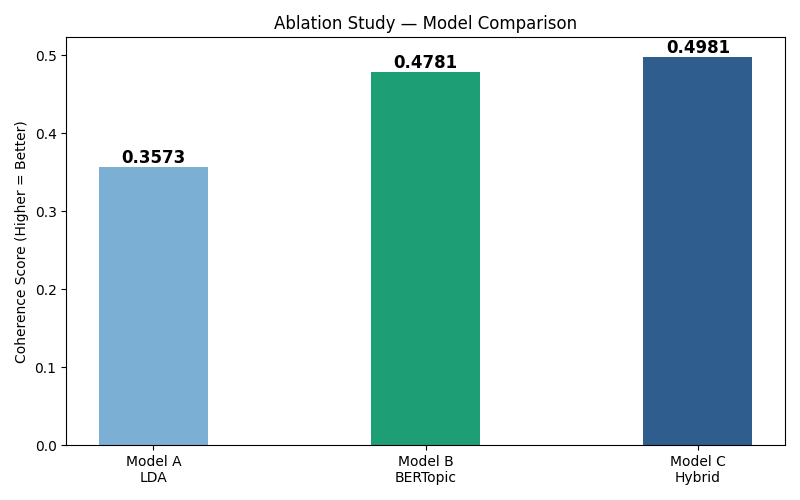
\includegraphics[width=\linewidth]{../graphs/ablation_graph.png}
    \caption{Ablation Study Results illustrating model improvements.}
    \label{fig:ablation}
\end{figure}

\section{Conclusion}
I successfully developed a Dynamic Trend \& Event Detector capable of interpreting massive news datasets. By transitioning from traditional probabilistic models to deep semantic architectures, I significantly improved topic coherence. The integration of semantic velocity and external validation through GDELT allowed the system to empirically differentiate a short-lived trend from a verified real-world event.

\begin{thebibliography}{9}
\bibitem{blei2003}
D. M. Blei, A. Y. Ng, and M. I. Jordan, ``Latent dirichlet allocation,'' \textit{Journal of Machine Learning Research}, vol. 3, pp. 993--1022, 2003.

\bibitem{grootendorst2022}
M. Grootendorst, ``BERTopic: Neural topic modeling with a class-based TF-IDF procedure,'' \textit{arXiv preprint arXiv:2203.05794}, 2022.

\bibitem{reimers2019}
N. Reimers and I. Gurevych, ``Sentence-BERT: Sentence embeddings using Siamese BERT-networks,'' \textit{arXiv preprint arXiv:1908.10084}, 2019.

\bibitem{misra2022}
R. Misra, ``News Category Dataset,'' \textit{Kaggle}, 2022.
\end{thebibliography}

\end{document}
